\documentclass[aspectratio=169]{beamer}
\mode<presentation>
%\usetheme{Warsaw}
%\usetheme{Goettingen}
\usetheme{Hannover}
%\useoutertheme{default}

%\useoutertheme{infolines}
\useoutertheme{sidebar}
\usecolortheme{dolphin}


\setbeamersize{sidebar width left=0pt} % to remove the sidebar
\beamertemplatenavigationsymbolsempty % To remove the navigation symbols on the bottom right.
\setbeamersize{text margin left=10mm,text margin right=10mm} % Specify margins

\usepackage{amsmath}
\usepackage{amssymb}
\usepackage{listings}
\usepackage{enumerate}
\usepackage{hyperref}
\hypersetup{
    colorlinks=true,
    linkcolor=blue,
    filecolor=magenta,      
    urlcolor=cyan,
}
 
\urlstyle{same}

%some bold math symbosl
\newcommand{\Cov}{\mathrm{Cov}}
\newcommand{\Var}{\mathrm{Var}}
\newcommand{\brho}{\boldsymbol{\rho}}
\newcommand{\bSigma}{\boldsymbol{\Sigma}}
\newcommand{\btheta}{\boldsymbol{\theta}}
\newcommand{\bbeta}{\boldsymbol{\beta}}
\newcommand{\bmu}{\boldsymbol{\mu}}
\newcommand{\bW}{\mathbf{W}}
\newcommand{\one}{\mathbf{1}}
\newcommand{\bH}{\mathbf{H}}
\newcommand{\by}{\mathbf{y}}
\newcommand{\bolde}{\mathbf{e}}
\newcommand{\bx}{\mathbf{x}}

\newcommand{\cpp}[1]{\texttt{#1}}

%--------------------------------------------------
\providecommand{\abs}[1]{\lvert#1\rvert}
\providecommand{\norm}[1]{\lVert#1\rVert}
\providecommand{\Blue}[1]{\textcolor{blue}{#1}}
\providecommand{\Red}[1]{\textcolor{red}{#1}}
\newcommand{\celsius}{\ensuremath{^\circ}C}
\newcommand\thfore{\mathord{\therefore}\,}
%--------------------------------------------

\title{Lecture 15. Tautology and Equivalence Rules}


\date{ }


\begin{document}
\frame[plain]{\titlepage}

\begin{frame}[plain]{When truth tables become impractical.}
  
  \begin{itemize}
   \item There is a limitation in using the truth table. Each time you add a new statement to a truth table, 
      you must double the number of rows. This makes truth table analysis unwieldy for all but the simplest
      examples.
   \item So, we will develop \Blue{a system of rules} for manipulating 
       propositional logic. 
   \item   Those rules will be useful for analyzing complex logical problems, especially
       where truth tables are impractical.
       %=   % which will allow us to make logical deduction formally.
  \end{itemize}

\end{frame}

\begin{frame}[plain]{}

    
 {\bf Practice 15.1.} Here's a question about playing Monopoly:
   \begin{quote}
     If you get more doubles than any other player, you will lose, 
     or if you lose, you must have bought the most properties.
   \end{quote}
     True or false?   
 %Levin, p199-200, Ex 3.1.2
 \pause
 \medskip
 
 The statement about monopoly is an example of a \Blue{tautology}, 
 a statement which is true on the basis of its \Red{logical form alone}. 
 Tautologies are always true but they don't tell us much about the world. 
 No knowledge about monopoly was required to determine that the statement 
 was true. In fact, it is equally true that 
 "If the moon is made of cheese, then Elvis is
   still alive, or if Elvis is still alive, 
   then unicorns have five legs."

\vspace{.in}
 
 \end{frame}

\begin{frame}[plain]{Tautology and Contradiction}%, and Contingency}

  Complete the truth table:
  
      \begin{center}
        \begin{tabular}{|c|c|c|c|}\hline
          $p$ & $\neg p$ &  $p\vee \neg p$ & $p\wedge \neg p$ \\ \hline
            	&  & & \\ \hline
               &   &  & \\ \hline            
        \end{tabular}
	\end{center}  
	\pause 

\begin{itemize}
 \item  A \Blue{tautology} is a statement that is {\bf always true} regardless of the truth values of the individual statements 
 substituted for its statement variables.
 %which is {\bf always true}.
    \begin{itemize}
     \item {\bf Example} $p\vee \neg p$ (I will get A or not A in this course)
    \end{itemize}
    A tautology is also called a \Blue{valid} statement.
  \item A \Blue{contradiction} is a statement that is {\bf always false} regardless of the truth values of the individual statements 
 substituted for its statement variables. 
   \begin{itemize}
     \item {\bf Example} $p\wedge \neg p$ (I will get A and not A in this course)
    \end{itemize}
 % \item A \Blue{contingency} is a statement which is neither a tautology 
  %      nor a contradiction. For example, a statement $p$.
 \end{itemize}
 
%     \pause
    
 %{\bf Example} Construct the truth table for  the statement
      %$(\neg p \wedge q) \rightarrow (q \oplus r)$ 
      % and determine whether the statement is 
      %tautology or not. %Exam2S22
     
\end{frame}



\begin{frame}[plain]{Logical Equivalence again}

In Lecture 14, we defined that two or more compound statements are  \Blue{logically equivalent}
if they have the same truth values in all possible cases.
\medskip

\Blue{Theorem 15.2.} The compound statements $P$ and $Q$ are  \Blue{logically equivalent} if
    $P \leftrightarrow Q$ is a tautology. 
    \begin{itemize}
      \item Why does this Theorem make sense? What if the truth values of $P$ and $Q$ are different?
      \pause 
      \item {\bf Notation} We write $P \leftrightarrow Q$ as $P \Red{\Leftrightarrow} Q$ to
         indicate the statement is tautology.
    \end{itemize}

 \vspace{.5in}
 

\end{frame}


\begin{frame}[plain]{Key Logical Equivalences}  

 {\bf De Morgan's Laws}
      \begin{enumerate}
        \item $\neg (p\wedge q) \Leftrightarrow \neg p \vee \neg q$
        \item $\neg (p\vee q) \Leftrightarrow \neg p \wedge \neg q$
      \end{enumerate}
 
 %{\bf Problem} Use a truth table to prove De Morgan's laws. \pause 
 %\medskip
 \pause 
\medskip

 {\bf Example 15.3.} 
   \begin{itemize}
    \item p:  The patient has migraines
    \item q: The patient has high blood pressure
   \end{itemize}


    De Morgan's law says that the following two English statements are
logically equivalent:
   \begin{itemize}
 %   \item It is not true that the patient has migraines or high blood pressure. \pause
    \item The patient does not have migraines or high blood pressure.
    \footnote{ 
     It is not true that the patient has migraines or high blood pressure.}
    \item The patient does not have migraines and does not have high blood pressure.
   \end{itemize}
\pause 
  % \item {\bf Example} Given the following statement
  %   \begin{quote}
  %     If Micah is \Blue{not} sick \Red{and} Micah is \Blue{not} tired, 
  %      then Micah can play.
  %   \end{quote}
  %   we can deduce the following using De Morgan's laws.
  %   \begin{quote}
  %     If it is \Blue{not} the case that Micah is sick \Red{or} tired, then
  %       Micah can play.
  %   \end{quote}
  
  {\bf Practice 15.4.} Are the statements, ``it will not rain and snow” 
   and ``it will not rain and it will not snow” logically equivalent?
%  Levin p202 Ex 3.1.3
  
\end{frame}



\begin{frame}[plain]{}
  
  \begin{center}
   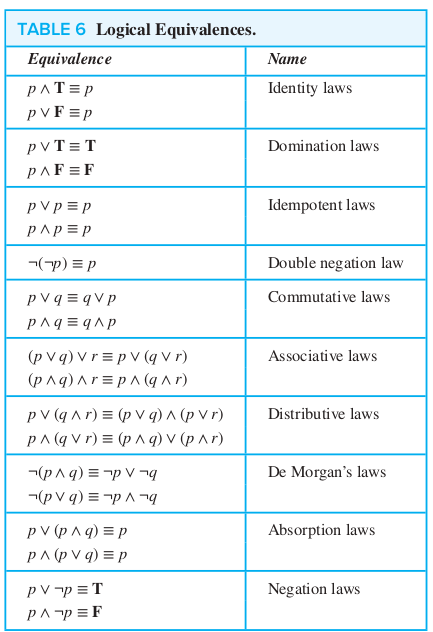
\includegraphics[height=8.7cm]{./img/lecture15-fig1.png}
  \end{center}  
 
\end{frame}



\begin{frame}[plain]{} 

  {\bf Practice 15.5.} What is the output of this computer program? Explain.
  \begin{center}
   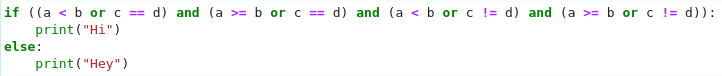
\includegraphics[height=1.5cm]{./img/lecture15-fig2.png}\pause
   
   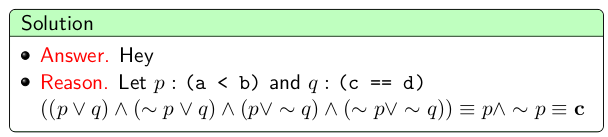
\includegraphics[height=2cm]{./img/lecture15-fig2-answer.png}
  \end{center}  
    
    \vspace{1in}
    
 % {\bf Exercise 15.6.} Ahmed, an intern of circuit design, 
 % thinks that the following circuit present in the design of the next-generation laptop 
 % can be
 % replaced by an \Blue{OR} gate. Is Ahmed right?
 % \begin{center}
 %  \includegraphics[height=2.5cm]{lecture14-fig5.png}
 %  %\includegraphics[height=1.5cm]{lecture14-fig5-answer.png}
 % \end{center}  
  
\end{frame}


\begin{frame}[plain]{}
  
  \begin{center}
   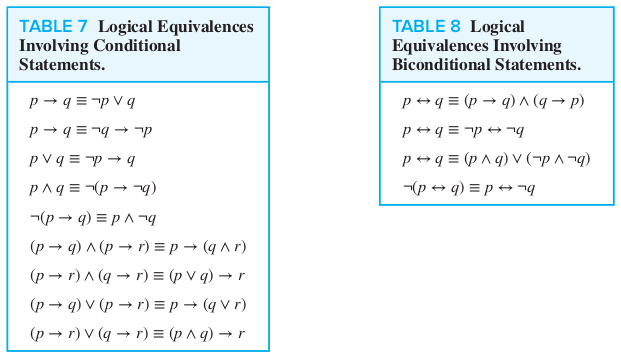
\includegraphics[height=6.5cm]{./img/lecture15-fig3.png}
  \end{center}  
   
  {\bf Example 15.6.} Rewrite the statement 
    “If a number is a multiple of 4, then it is even” equivalently without using the logical
    connective ``if".
    %Answer: “A number is not a multiple of 4 or (else) it is even.”
  
  
\end{frame}


\begin{frame}[plain]{Constructing New Logical Equivalences}
 The logical equivalences on the previous page can be used to construct additional logical equivalences.
 %The
%reason for this is that a proposition in a compound statement can be replaced by another compound
%statement that is logically equivalent to it without changing the truth value of the original
%compound statement.
\smallskip

  {\bf Example 15.7.} Show that $\neg (p\rightarrow q)$ and $p\wedge \neg q$ are logically equivalent
     without using a truth table. %Rosen's book p30 EX 7
     \pause 
     
     \begin{itemize}
       \item {\bf Solution} 
          \begin{eqnarray*}
             \neg (p\rightarrow q) &\Leftrightarrow& \neg (\neg p\vee q) \ \ \ \ \ \ \mbox{by Conditional identities}\\
                &\Leftrightarrow& \neg (\neg p) \wedge \neg q \ \ \ \  \mbox{by De Morgan's laws} \\
                &\Leftrightarrow& p \wedge \neg q \ \ \ \ \ \ \ \ \ \ \ \mbox{by Double negation} 
          \end{eqnarray*}
     \end{itemize}
 
 \vspace{.5in}
 
\end{frame}



\begin{frame}[plain]{ }

{\bf Practice 15.8.}  
  Fill in the reasons in the following proof sequence. Make sure you indicate which 
     equivalence rule is used.
     \begin{center}
       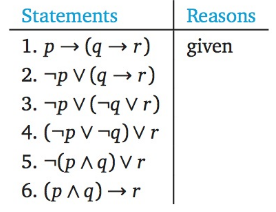
\includegraphics[height=4cm]{./img/lecture15-fig4.png}
     \end{center}
 \vspace{.5in}

 \end{frame}
 

 \begin{frame}[plain]{}
 
 
  {\bf Practice 15.9.}  Show that $\neg (p\vee (\neg p\wedge q))$ and $\neg p \wedge \neg q$ are logically
       equivalent by developing a series of logical equivalence.\ \ 
 
 \vspace{2in}
 
\end{frame}

%%%%%%%%%%
\end{document}
%%%%%%%%%%
 

\end{document}
%--------------------------------------------------

    


    
